
After acquiring the models from a set of training grasps, we present the robot with a test (query) object. The goal is to find a generalisation of the training grasp that is likely according to all of the model types simultaneously. First of all, we obtain a point cloud for the test object, and thus an object model. We then combine every contact model with that object model, so as to obtain a set of {\em query densities}, one for each link with a contact model defined for the example grasp. The $i$-th query density $\qd_i$ is a density modelling where the $i$-th link can be placed, in the equilibrium state, with respect to the surface of a new object. 

From the query densities, a candidate equilibrium grasp state is generated . This is then augmented with a reach to grasp trajectory that finishes close to the candidate equilibrium grasp state. Finally we refine the equilibrium grasp and reach to grasp by performing a simulated annealing search in the space of equilibrium state wrist poses and hand configurations, so as to maximise the grasp likelihood. We repeat the entire process many times. This procedure generates many possible grasps, ranked likelihood. We give details below.

\subsection{Query Density}

A query density \eqref{eq:qd} is expressed, for a hand link and an object model, as a density for the pose of that hand link relative to the object. Intuitively the query density encourages a finger link to make contact with the object at locations that have similar local surface curvature to that in the training example. Specifically, we use $K_{Q_i}$ kernels centred on the set of weighted finger link poses:
\begin{equation}
\qd_i(s) \simeq \sum^{K_{Q_i}}_{j=1} w_{ij} \mathcal{N}_3(p|{\hat{p}_{ij}}, \sigma_{p}) \Theta(q|{\hat{q}_{ij}}, \sigma_{q})%, \quad i = 1, ..., N_L
\label{eq:qd.approx}
\end{equation}
with $j$-th kernel centre $({\hat{p}_{ij}}, {\hat{q}_{ij}}) = \hat{s}_{ij}$, and weights are normalised $\sum_j w_{ij} = 1$. When a test object is presented, a set of query densities $\mathcal{Q}^g$ is calculated for the equilibrium state for each training grasp $b$ for the grasp type $g$. The set $\mathcal{Q}^g_b =\{\qd_{b,i}^g\}$ has $N^g_Q=N^g_M$ members, one for each contact model $M_i^g$ in $\mathcal{M}^g$. We estimate the query density using a Monte Carlo procedure detailed in Alg.\ref{alg:mc}.

\begin{algorithmbox}[floatplacement=t,float,fontupper=\small,label={alg:mc}]{Pose sampling ($\cm_i${,} $\om$)}
\begin{minipage}{\linewidth}\begin{tabbing}%
For \= samples $j=1$ to $K_{Q_i}$\\
  \> Sample $(\hat{v}_j, \hat{r}_j) \sim \om(v, r)$\\
  \> Sample from conditional density $(\hat{u}_{ij}) \sim \cm_i(u|\hat{r}_j)$\\
	\> Compute sample weight $w_{ij} = \cm_i(\hat{r}_j)$\\
	\> $\hat{s}_{ij} = \hat{v}_{j} \circ \hat{u}_{ij}$ \\
	\> separate $\hat{s}_{ij}$ into position $\hat{p}_{ij}$ and quaternion $\hat{q}_{ij}$\\
return $\{  (\hat{p}_{ij}, \hat{q}_{ij}, w_{ij} ) \}, \,  \forall j $
\end{tabbing}\end{minipage}
\end{algorithmbox}

\subsubsection{Equilibrium Grasp Generation} 
One query densities have been created for the new object for each training example, an initial set of equilibrium state grasps is generated for each grasp type $g$. For each new initial equilibrium grasp of a particular grasp type we proceed as follows. First an example grasp is selected at random. Then a finger link is selected at random. This ‘seed’ link indexes its query density $\qd_i^g$. A link pose $s_i$ is then sampled from that query density. Then an equilibrium state hand configuration $h^e_c$ is sampled from $\hc^g$. Together the seed link and the hand configuration define a complete equilibrium state hand pose $h$ in the workspace via forward kinematics. This is an initial `seed' grasp, which will subsequently be refined. A large set of such initial solutions is generated, where $h_e^g(j)=(h_w^{e}(j) , h_c^{e}(j) , h_m^{e}(j))$ means the $j^{th}$ initial solution for  grasp type $g$. 

\subsection{Reach to Grasp Generation}
Given an equilibrium grasp, a reach to grasp trajectory is selected and adapted to maximise the chance of reaching that equilibrium grasp state. Specifically, the reach to grasp model $(h_w^{0:e} , h_c^{0:e} , h_m^{0:e})$ which has a final hand configuration state $h^e_c$ with the smallest Euclidean distance in joint space to the $j^th$ equilibrium grasp $h_e^g(j)$ is paired with that grasp. To align it, the wrist trajectory $h_w^{0:e}$ is defined relative to the frame $h_w^{e}(j)$. Then the configuration trajectory $h_c^{0:e}$ is warped (Fig\ref{fig:reaches}) with a first-order lag function so that it smoothly shifts from $h_c^{0}$ to $h_c^{e}(j)$. Having generated an initial solution set $\mathcal{H}^{1}$ stages of optimisation and selection are interleaved.

\begin{figure}

 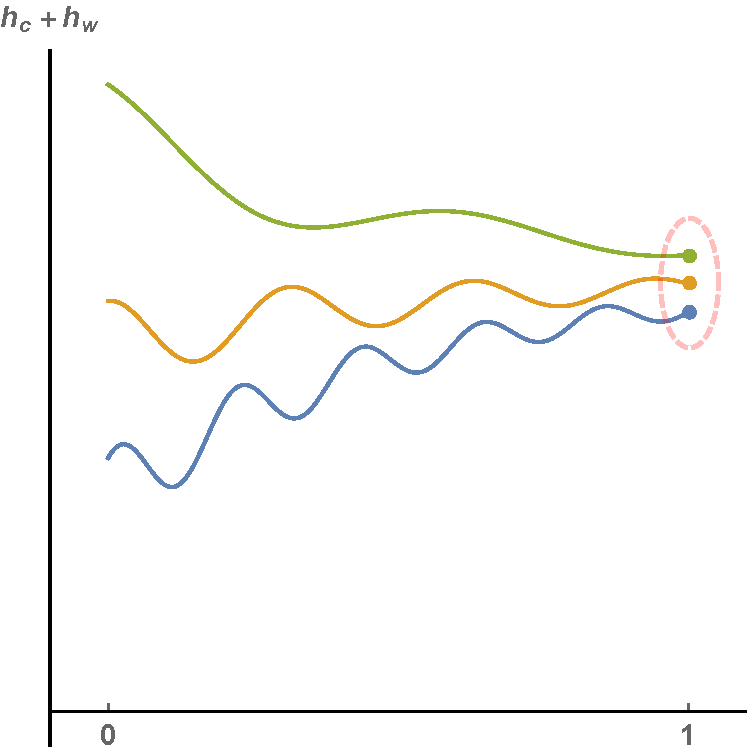
\includegraphics[width=0.45\linewidth]{images/config_space_plots/2_basin_of_attraction}
  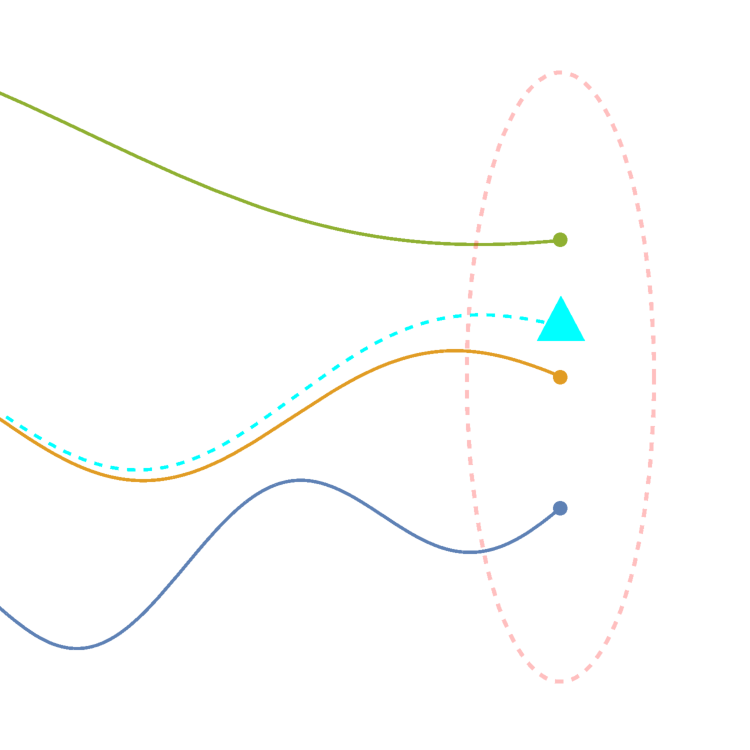
\includegraphics[width=0.45\linewidth]{images/config_space_plots/5_trajectory_adaptation}
 \caption{{We acquire set of trajectories that, associated with a model of the final equilibrium grasp state, form an attractor basin around that state.}}
  \label{fig:reaches}
\end{figure}

\subsubsection{Grasp Optimisation Steps}
The objective of the grasp optimisation steps is, given a candidate grasp and a grasp model $g$, to find a grasp that maximises the product of the likelihoods of the query densities and the hand configuration density
\begin{align}
\argmax{(h)}  \mathcal{L}^g(h) & \\
 = \argmax{(h)}  \mathcal{L}^g_\hc(h) \mathcal{L}^g_\qd(h) \\
 = \argmax{(h_w, h_c)}   \hc^{g}(h_c) \prod_{\qd_i^g \in \mathcal{Q}^g} \qd_i^g\left(k_{i}^{\mathrm{for}}\left(h_w, h_c\right)\right)
\label{eq:grasping.product}
\end{align}
where ${\cal L}^g(h)$ is the overall likelihood, where $\hc^g(h_c)$ is the hand configuration model~\eqref{eq:hc}, $\qd_i^g$ are query densities~\eqref{eq:qd.approx}. Thus whereas each initial grasp is generated using only a single query density, grasp optimisation requires evaluation of the grasp against all query densities. It is only in this improvement phase that all query densities must be used.
 Improvement is by simulated annealing (SA) \cite{kirkpatrick83optimizationby}. The SA temperature $T$ is declined linearly from $T_{1}$ to $T_{K}$ over the $K$ steps. In each time step, one step of simulated annealing is applied to every grasp $m$ in $\mathcal{H}^k$.